\section{Results} \label{sec:results}

\subsection{Simulation} \label{sec:results_sim}

A subset of all settings was kept constant for all simulations. The instrument settings are presented in Table \ref{tab:inst_settings} and the settings for the \gls{sssb} in Table \ref{tab:sssb_settings}. The specific values were chosen in order to mimic the scenario in \cite{Pajusalu2019CharacterizationMapping}.

\begin{table}[htb]
    \centering
    \caption{Instrument Settings}
    \label{tab:inst_settings}
    \begin{tabular}{l|l}
        \textbf{Parameter Name} & \textbf{Value} \\ \hline
        res       & $\SI{2464}{} \times \SI{2054}{}$   \\
        pix\_l        & \SI{3.45}{\micro\meter}     \\
        focal\_l       & \SI{230}{\milli\meter}     \\
        aperture\_d     &  \SI{4}{\centi\meter} \\
        wavelength  & \SI{550}{\nano\meter} \\
        quantum\_eff & \SI{0.25}{} \\
        color\_depth & \SI{8}{\bit}
    \end{tabular}
\end{table}

\begin{table}[htb]
    \centering
    \caption{\gls{sssb} settings.}
    \label{tab:sssb_settings}
    \begin{tabular}{l|l}
        \textbf{Parameter Name} & \textbf{Value} \\ \hline
        a       & \SI{1.644641475071416}{\astronomicalunit}   \\
        e        & \SI{3.838774437558215E-01}{}\\
        i       & \SI{3.408231185574551E+00}{\radian}\\
        P &  \SI{7.703805051391988E+02}{\radian} \\
        omega  & \SI{3.192958853076784E+02}{\radian} \\
        Omega & \SI{7.320940216397703E+01}{\radian} \\
        M & \SI{1.967164895190036E+02}{\radian} \\
        date & 2017-08-19T00:00:00.000 \\
        rotation\_rate & \SI{8133.48}{\per\second} \\
        albedo & \SI{0.15}{} \\
        max\_dim & \SI{512}{}
    \end{tabular}
\end{table}

\begin{table}[htb]
    \centering
    \caption{Simulation settings.}
    \label{tab:sim_settings}
    \begin{tabular}{l|l}
        \textbf{Parameter Name} & \textbf{Value} \\ \hline
        duration       & \SI{120}{\second}   \\
        encounter\_date & 2017-08-15T12:00:00.000\\
        frames       & \SI{120}{}     \\
        relative\_velocity     &  \SI{10}{\kilo\meter\per\second} \\
        with\_terminator  & \SI{0}{} \\
        with\_sunnyside & \SI{1}{} \\
        timesampler\_mode & \SI{1}{} \\
        exposure & \SI{0}{} \\
        samples & \SI{48}{} \\
        device & \gls{gpu} \\
        tile\_size & \SI{512}{} \\
        with\_clipping & \SI{1}{}
    \end{tabular}
\end{table}


\subsection{Compression} \label{sec:results_comp}
The \gls{sispo} software package was used to study the effects of compression in different scenarios. The scenarios are presented in Table \ref{tab:sim_params}. Mainly the effects of two parameters were studied, the size of an \gls{sssb} and the flyby distance. Comparison of the different compression algorithms is based on several output parameters. The data size of the compressed image series, the number of points that could be reconstructed, the number of vertices that could be reconstructed and the number of faces. These outputs relate well to the level of detail of the rendered images, since \gls{sfm} algorithms rely on surface details for reconstruction.


\begin{table}[htb]
\caption{Simulation parameters}
\label{tab:sim_params}
\begin{tabular}{l|lll}
ID      & \gls{sssb} Size \SI{}{\kilo\meter} & Encounter Distance \SI{}{\kilo\meter} & Compression Method      \\
Default & 1                                                                                                        & 400                                                                                          & png                     \\
1       & 1                                                                                                        & 400                                                                                          & jpeg2000: quality 1000  \\
2       & 1                                                                                                        & 400                                                                                          & jpeg2000: quality 100   \\
3       & 1                                                                                                        & 400                                                                                          & jpeg2000: quality 10    \\
4       & 1                                                                                                        & 100                                                                                          & png                     \\
5       & 1                                                                                                        & 100                                                                                          & jpeg2000 : quality 1000 \\
6       & 1                                                                                                        & 100                                                                                          & jpeg2000: quality 100   \\
7       & 1                                                                                                        & 100                                                                                          & jpeg200: quality 10     \\
8       & 1                                                                                                        & 1000                                                                                         & png                     \\
9       & 1                                                                                                        & 1000                                                                                         & jpeg2000 : quality 1000 \\
10      & 1                                                                                                        & 1000                                                                                         & jpeg2000 : quality 100  \\
11      & 1                                                                                                        & 1000                                                                                         & jpeg2000 : quality 10   \\
12      & 10                                                                                                       & 400                                                                                          & png                     \\
13      & 10                                                                                                       & 400                                                                                          & jpeg2000 : quality 1000 \\
14      & 10                                                                                                       & 400                                                                                          & jpeg2000 : quality 100  \\
15      & 10                                                                                                       & 400                                                                                          & jpeg2000 : quality 10   \\
16      & 0.1                                                                                                      & 400                                                                                          & png                     \\
17      & 0.1                                                                                                      & 400                                                                                          & jpeg2000 : quality 1000 \\
18      & 0.1                                                                                                      & 400                                                                                          & jpeg2000 : quality 100  \\
19      & 0.1                                                                                                      & 400                                                                                          & jpeg2000 : quality 10  
\end{tabular}
\end{table}

\subsection{Image Quality Comparison}
To compare the image quality after different levels of compression, a specific image is selected which is compressed to different levels. Since reconstruction is mostly influenced by surface features, a scene with a distance of \SI{50}{\kilo\meter} was selected for comparison. To better show the artefacts created by compression, the area highlighted by the red box in Figure \ref{fig:img_quality_frame} was studied up closer.

\begin{figure}[htb]
    \centering
    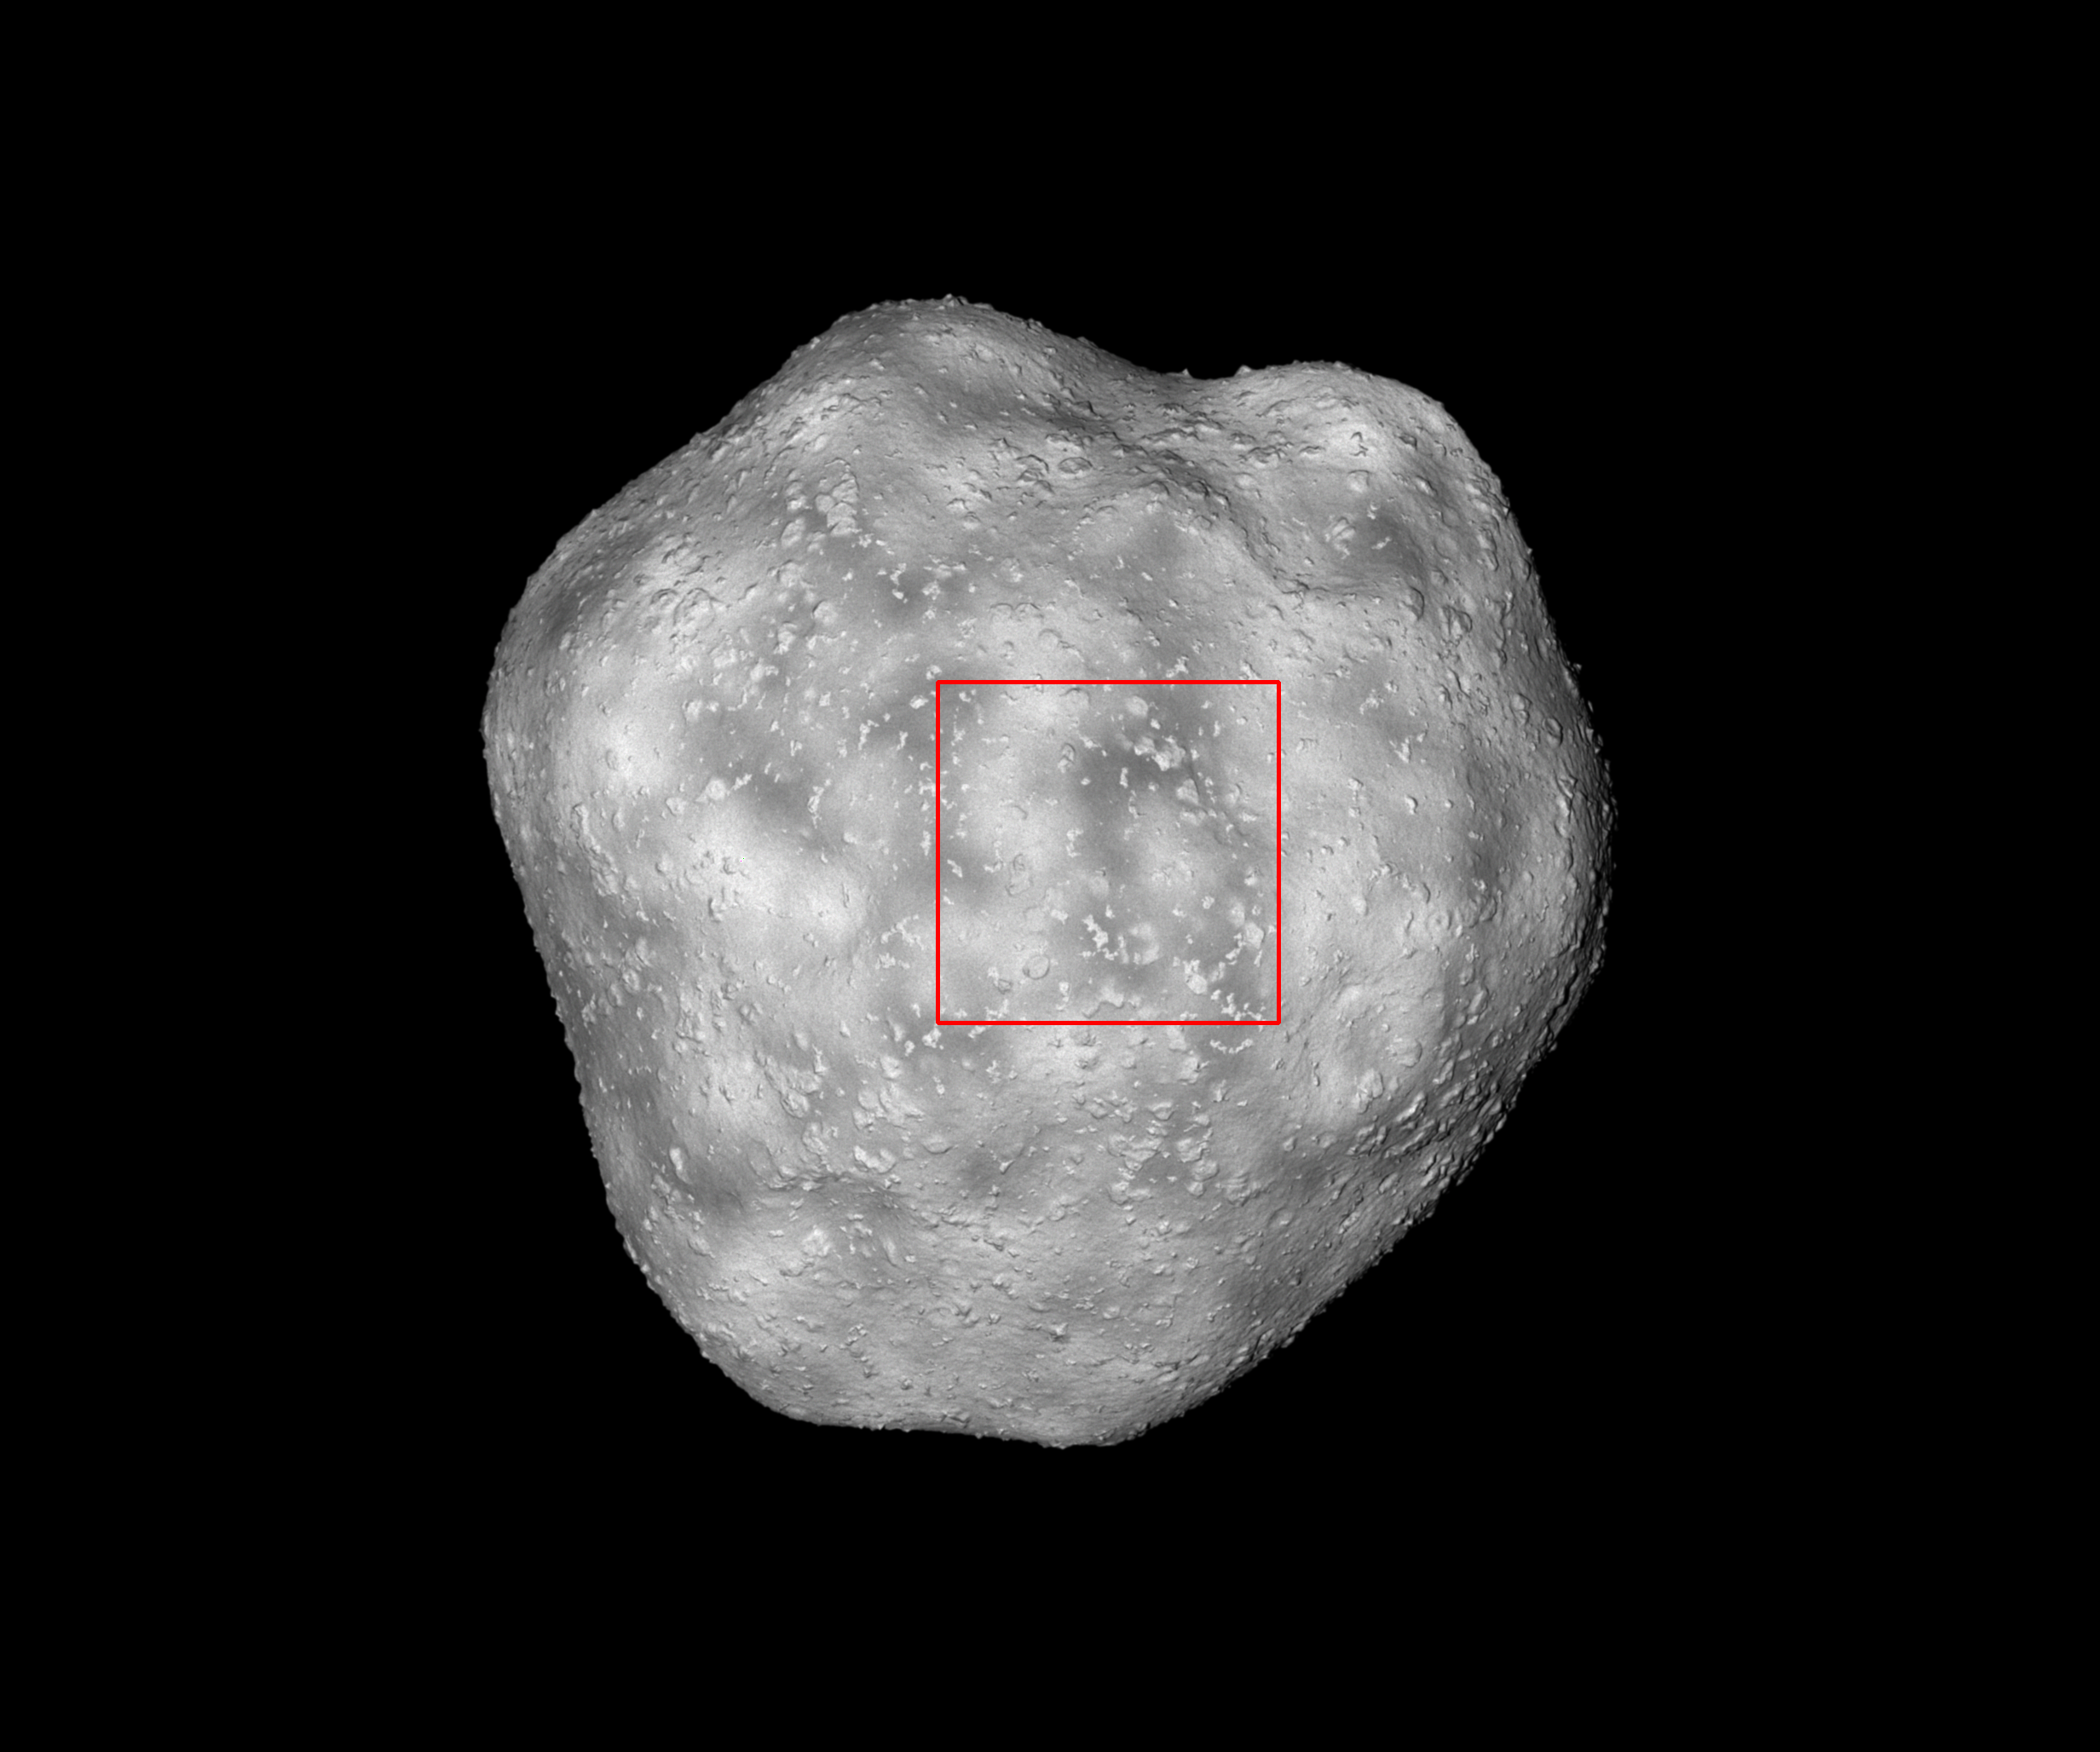
\includegraphics[width=\textwidth]{doc/thesis/0_figures/quality_compare/jp2_1000_frame.png}
    \caption{Scene used for quality comparison. Highlighted in red is the area studied up closer.}
    \label{fig:img_quality_frame}
\end{figure}

Figure \ref{fig:img_quality_comp}

\begin{figure}[htb]
    \centering
        \begin{subfigure}[b]{0.47\textwidth}
            \centering
                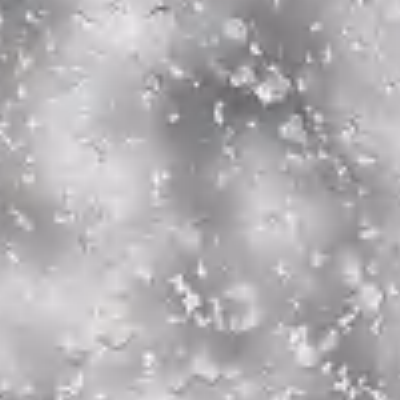
\includegraphics[width=\textwidth]{doc/thesis/0_figures/quality_compare/jp2_1_center.png}
            \caption{Quality 1.}
            \label{fig:img_quality_1}
        \end{subfigure}
        \begin{subfigure}[b]{0.47\textwidth}
            \centering
                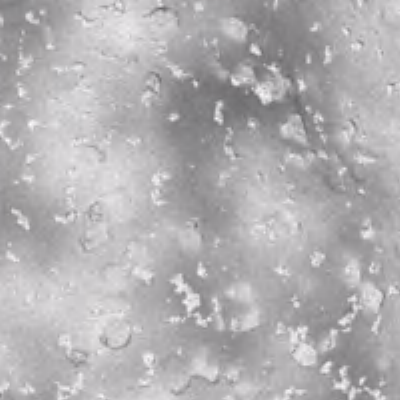
\includegraphics[width=\textwidth]{doc/thesis/0_figures/quality_compare/jp2_4_center.png}
            \caption{Quality 4.}
            \label{fig:img_quality_4}
        \end{subfigure}
        \\
        \begin{subfigure}[b]{0.47\textwidth}
            \centering
                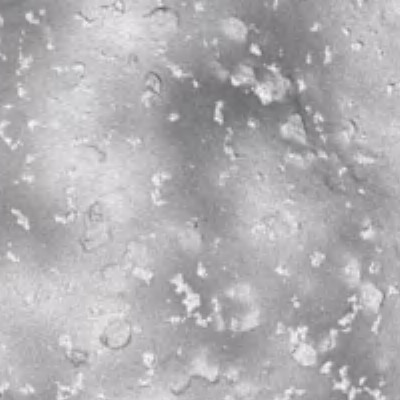
\includegraphics[width=\textwidth]{doc/thesis/0_figures/quality_compare/jp2_5_center.png}
            \caption{Quality 5.}
            \label{fig:img_quality_5}
        \end{subfigure}
        \begin{subfigure}[b]{0.47\textwidth}
            \centering
                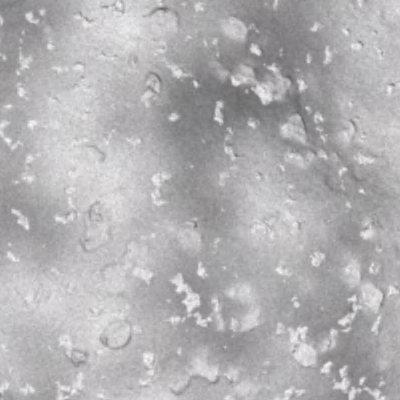
\includegraphics[width=\textwidth]{doc/thesis/0_figures/quality_compare/jp2_10_center.png}
            \caption{Quality 10.}
            \label{fig:img_quality_10}
        \end{subfigure}
        \\
        \begin{subfigure}[b]{0.47\textwidth}
            \centering
                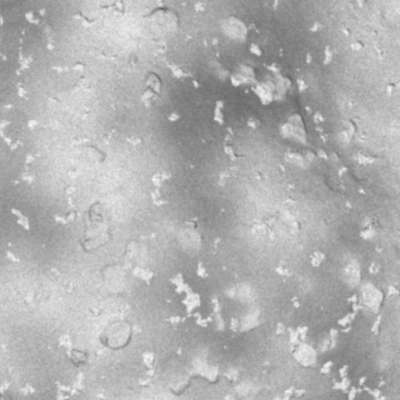
\includegraphics[width=\textwidth]{doc/thesis/0_figures/quality_compare/jp2_100_center.png}
            \caption{Quality 100.}
            \label{fig:img_quality_100}
        \end{subfigure}
        \begin{subfigure}[b]{0.47\textwidth}
            \centering
                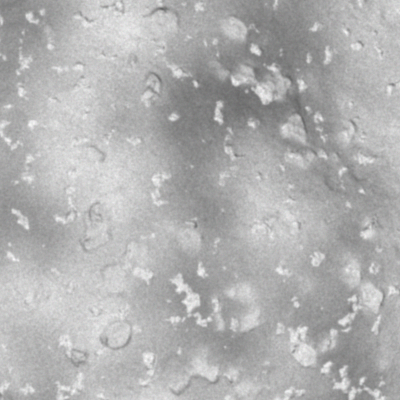
\includegraphics[width=\textwidth]{doc/thesis/0_figures/quality_compare/jp2_1000_center.png}
            \caption{Quality 1000.}
            \label{fig:img_quality_1000}
        \end{subfigure}
    \caption{Comparison of images with different level of compression using \gls{jpeg}2000.}
    \label{fig:img_quality_comp}
\end{figure}

\subsection{Different Distances}
Through procedural terrain generation, \gls{sispo} produces results for a large range of encounter distances. Example images with different surface distances and \gls{sssb} sizes are shown in Figure \ref{fig:img_procedural_10k}.

\begin{figure}[htb]
    \centering
        \begin{subfigure}[b]{0.75\textwidth}
            \centering
                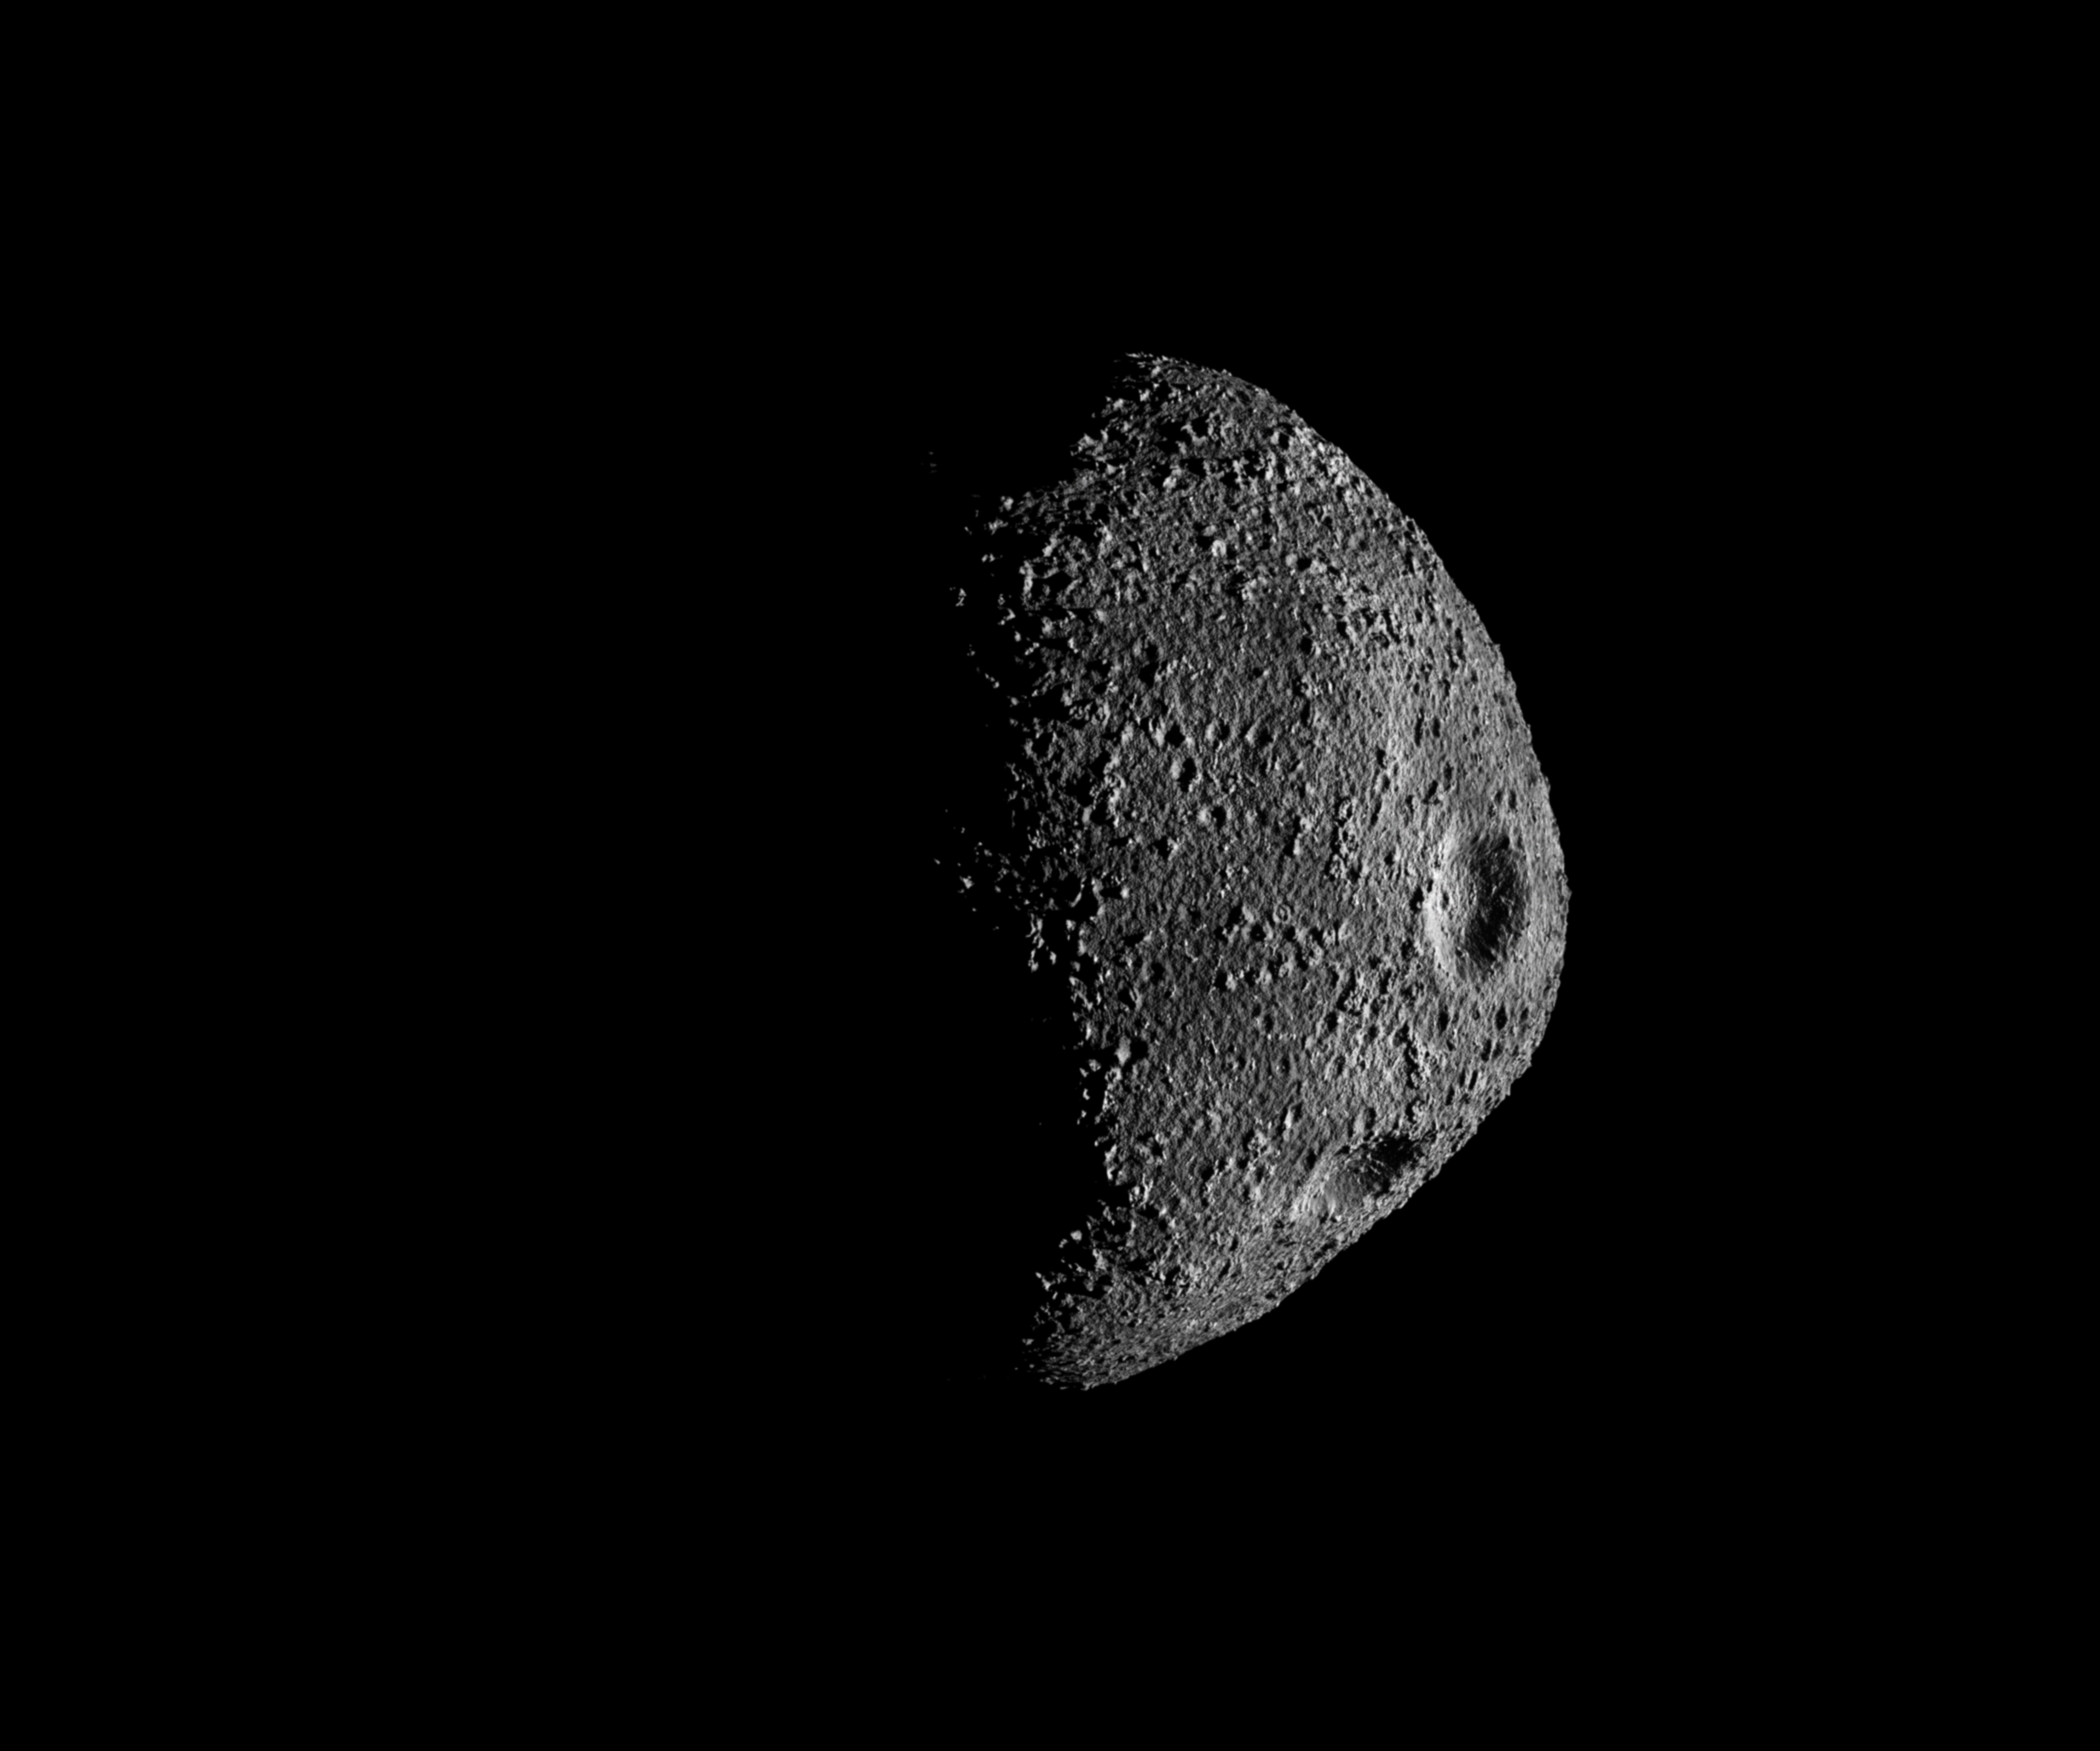
\includegraphics[width=\textwidth]{doc/thesis/0_figures/procedural_terrain/50_10_Inst_2017-08-15T115755-845000.png}
            \caption{\SI{566}{\kilo\meter}.}
            \label{fig:img_procedural_500}
        \end{subfigure}
        \\
        \begin{subfigure}[b]{0.75\textwidth}
            \centering
                \includegraphics[width=\textwidth]{doc/thesis/0_figures/procedural_terrain/50_10_Inst_2017-08-15T115855-260000.png}
            \caption{\SI{106}{\kilo\meter}.}
            \label{fig:img_procedural_100}
        \end{subfigure}
    \caption{Surface of a \SI{10}{\kilo\meter} \gls{sssb} at the given distances.}
    \label{fig:img_procedural_10k}
\end{figure}

It is visible from Figure \ref{fig:img_procedural_10k} that surface features and details do not degrade visually. In addition, moving closer reveals more details, such as tiny bumps between larger structures which are not visible from larger distances.


\subsection{Composition}
The composition process uses raw images rendered with Blender and produces photometrically calibrated images. An example set of four images consisting of two images before and after calibration is shown in Figure \ref{fig:composition_before_after}. All four images were converted to \SI{8}{\bit} images. Two effects can be seen. First, the original images differ in there overall brightness. This difference is removed by the calibration. Secondly, images become brighter by the calibration process. 

\begin{figure}[htb]
    \centering
        \begin{subfigure}[b]{0.48\textwidth}
            \centering
                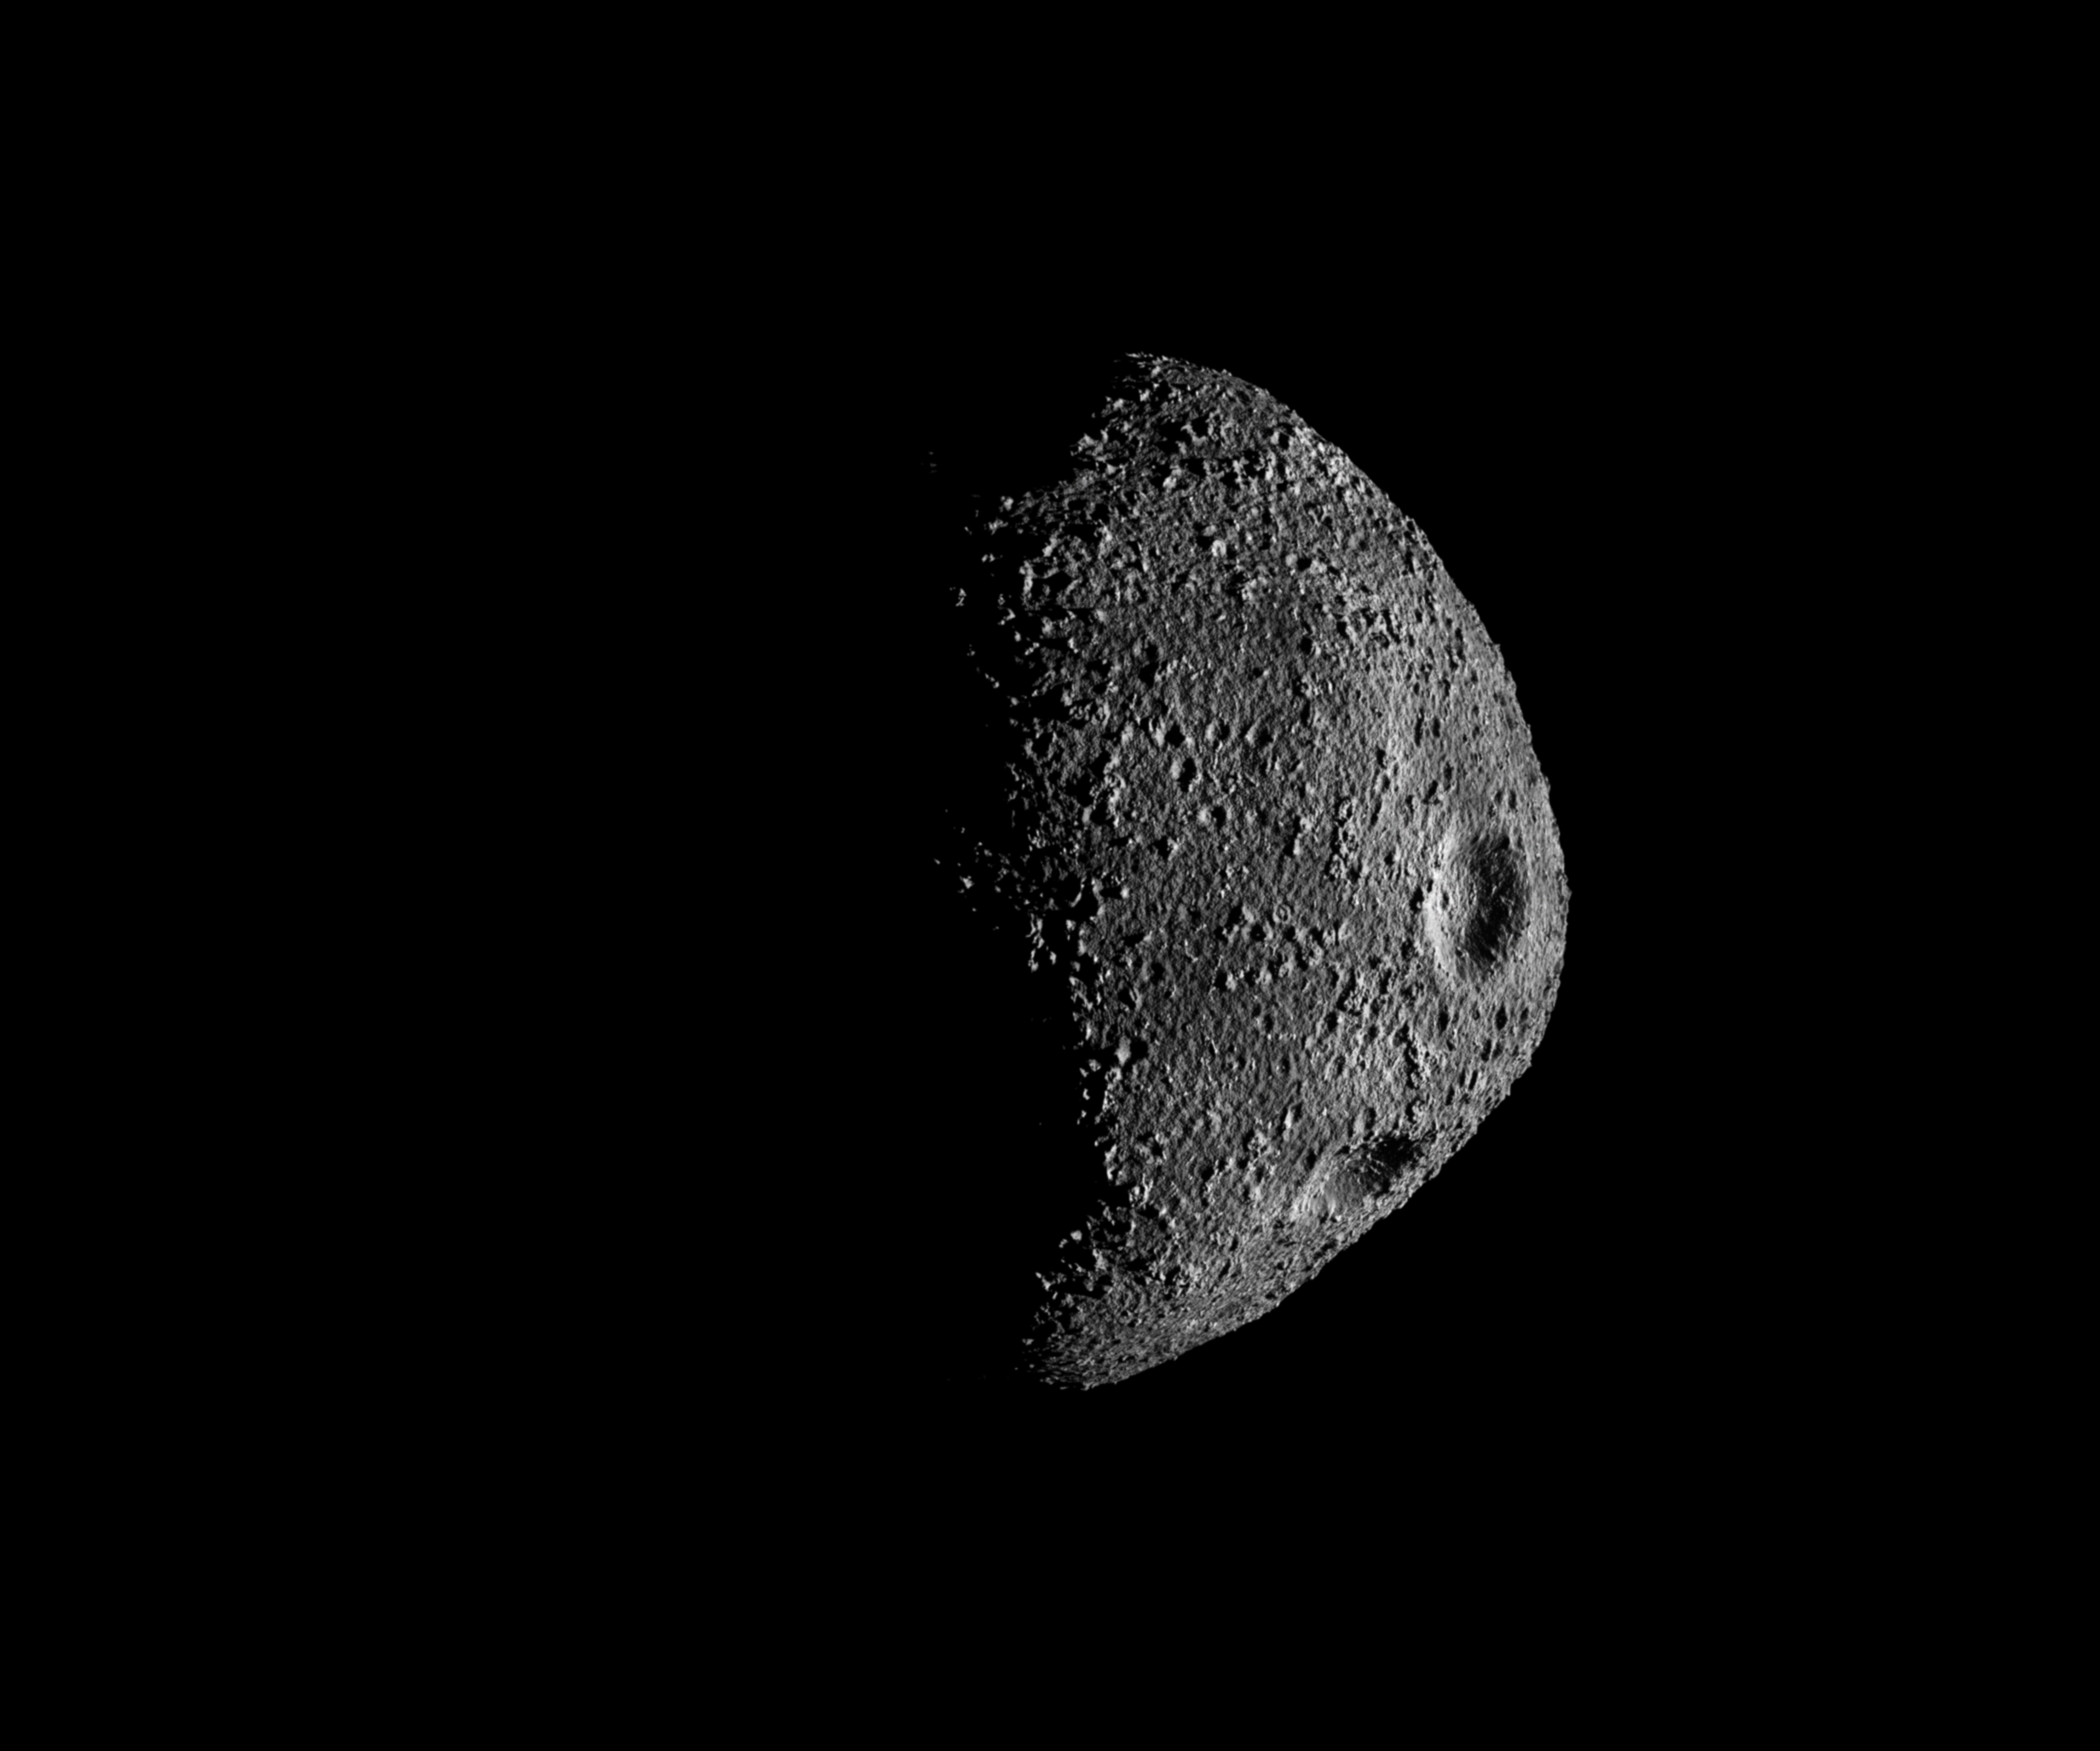
\includegraphics[width=\textwidth]{doc/thesis/0_figures/procedural_terrain/50_10_Inst_2017-08-15T115755-845000.png}
                \caption{Image 1 before calibration.}
                \label{fig:composition_before_1}
        \end{subfigure}
        \begin{subfigure}[b]{0.48\textwidth}
            \centering
                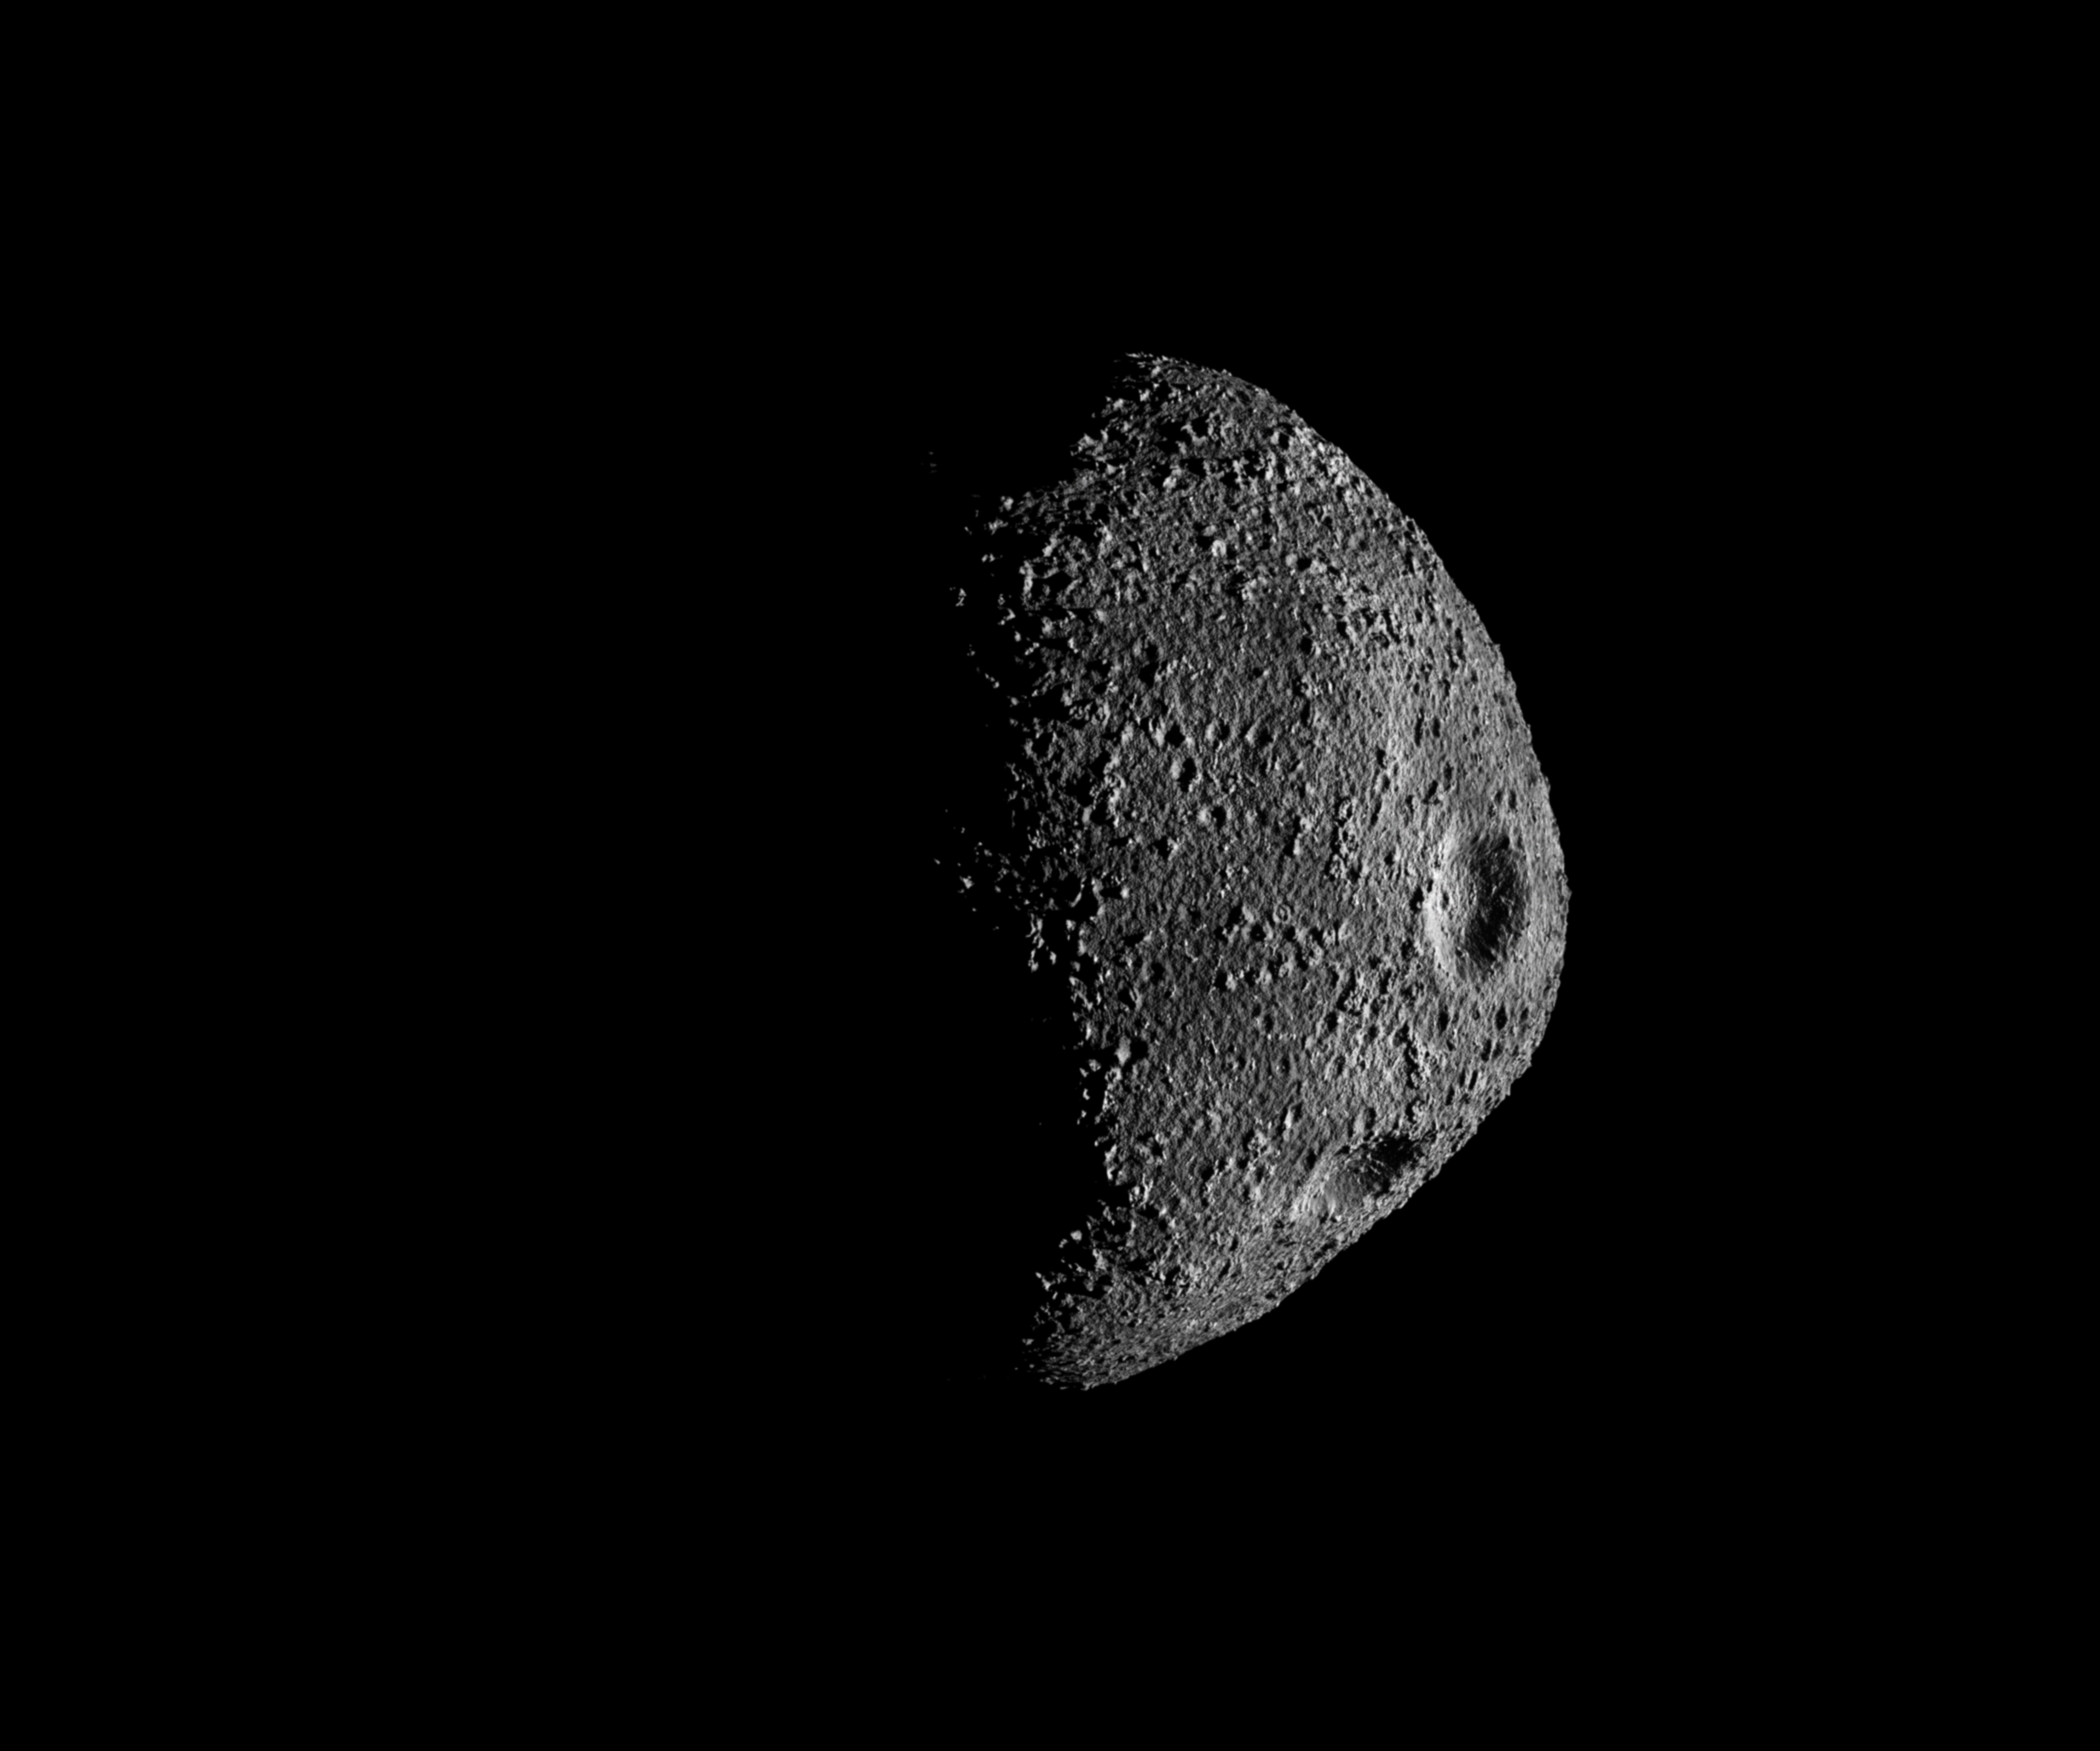
\includegraphics[width=\textwidth]{doc/thesis/0_figures/procedural_terrain/50_10_Inst_2017-08-15T115755-845000.png}
                \caption{Image 2 before calibration.}
                \label{fig:composition_before_2}
        \end{subfigure}
        \\
        \begin{subfigure}[b]{0.48\textwidth}
            \centering
                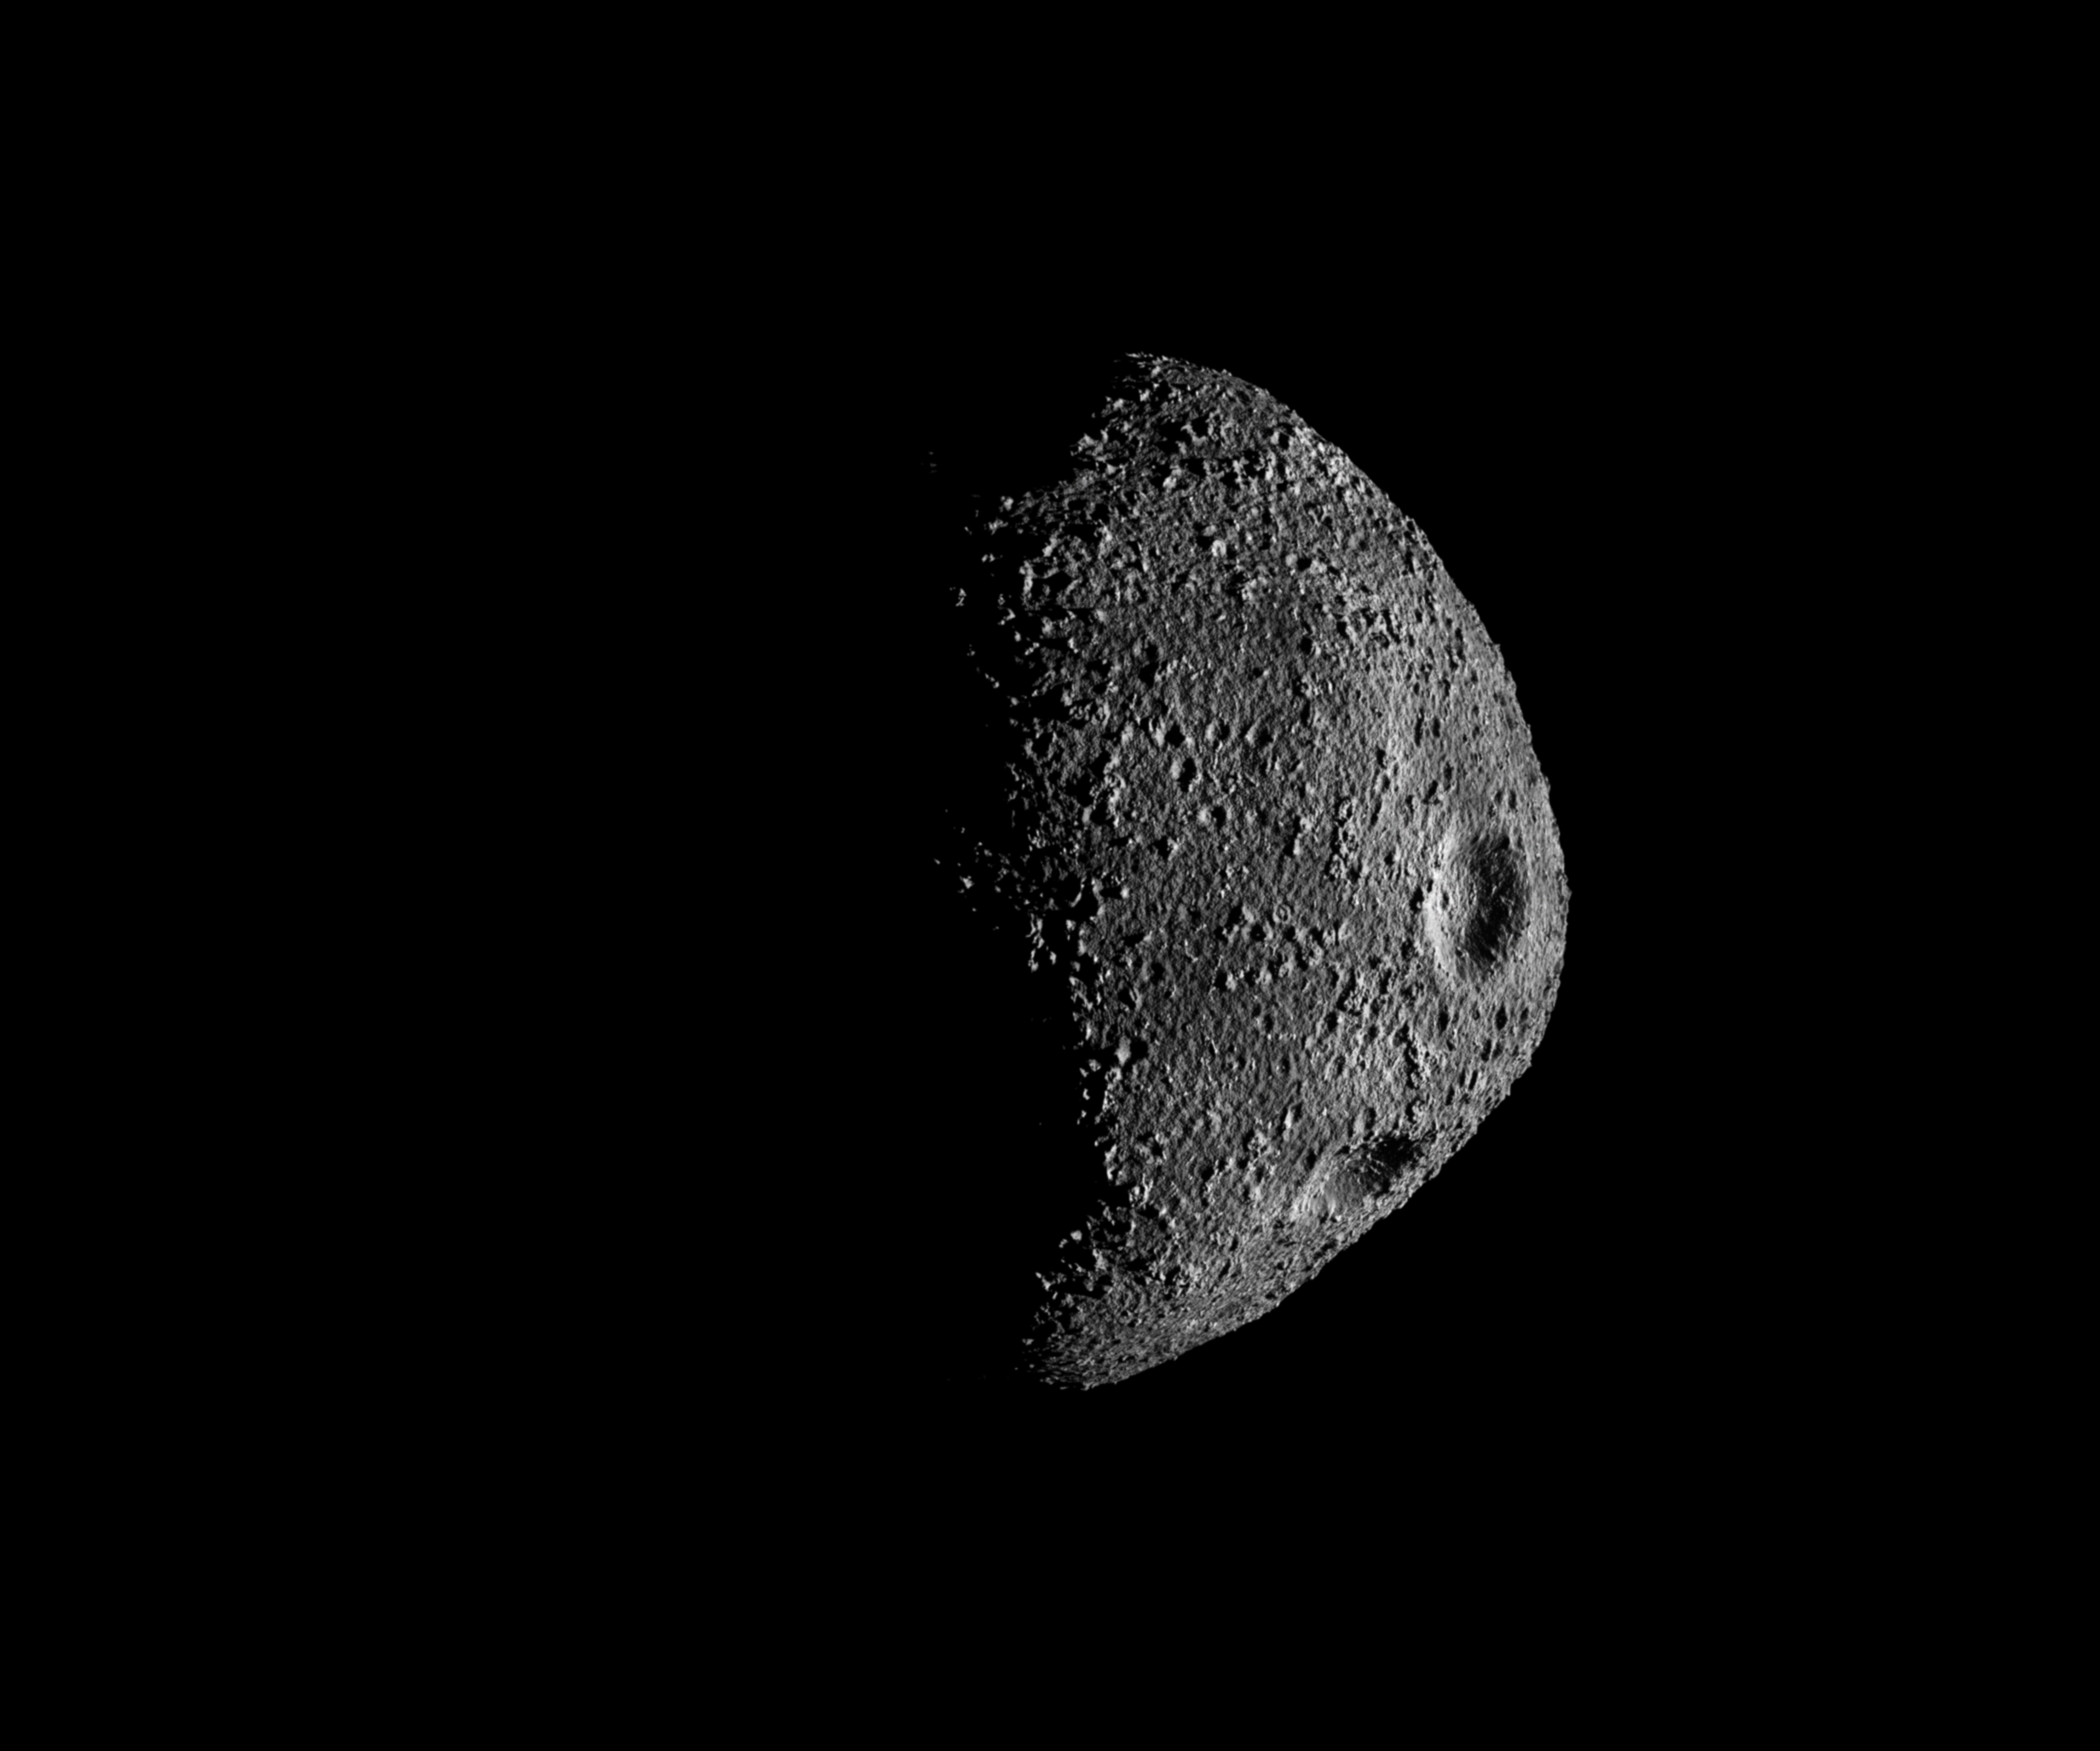
\includegraphics[width=\textwidth]{doc/thesis/0_figures/procedural_terrain/50_10_Inst_2017-08-15T115755-845000.png}
                \caption{Image 1 after calibration.}
                \label{fig:composition_after_1}
        \end{subfigure}
        \begin{subfigure}[b]{0.48\textwidth}
            \centering
                \includegraphics[width=\textwidth]{doc/thesis/0_figures/procedural_terrain/50_10_Inst_2017-08-15T115855-260000.png}
                \caption{Image 2 after calibration.}
                \label{fig:composition_after_2}
        \end{subfigure}
        \caption{Two images of a flyby, image 2 is one second after image 1, before and after the composition process. The nucleus is much brighter than background stars thus no stars visible in these images after calibration.}
        \label{fig:composition_before_after}
\end{figure}


\subsection{Rendering Problems}
When using a \SI{10}{\kilo\meter} \gls{sssb}, 
\begin{figure}[htb]
    \centering
        \begin{subfigure}[b]{0.75\textwidth}
            \centering
                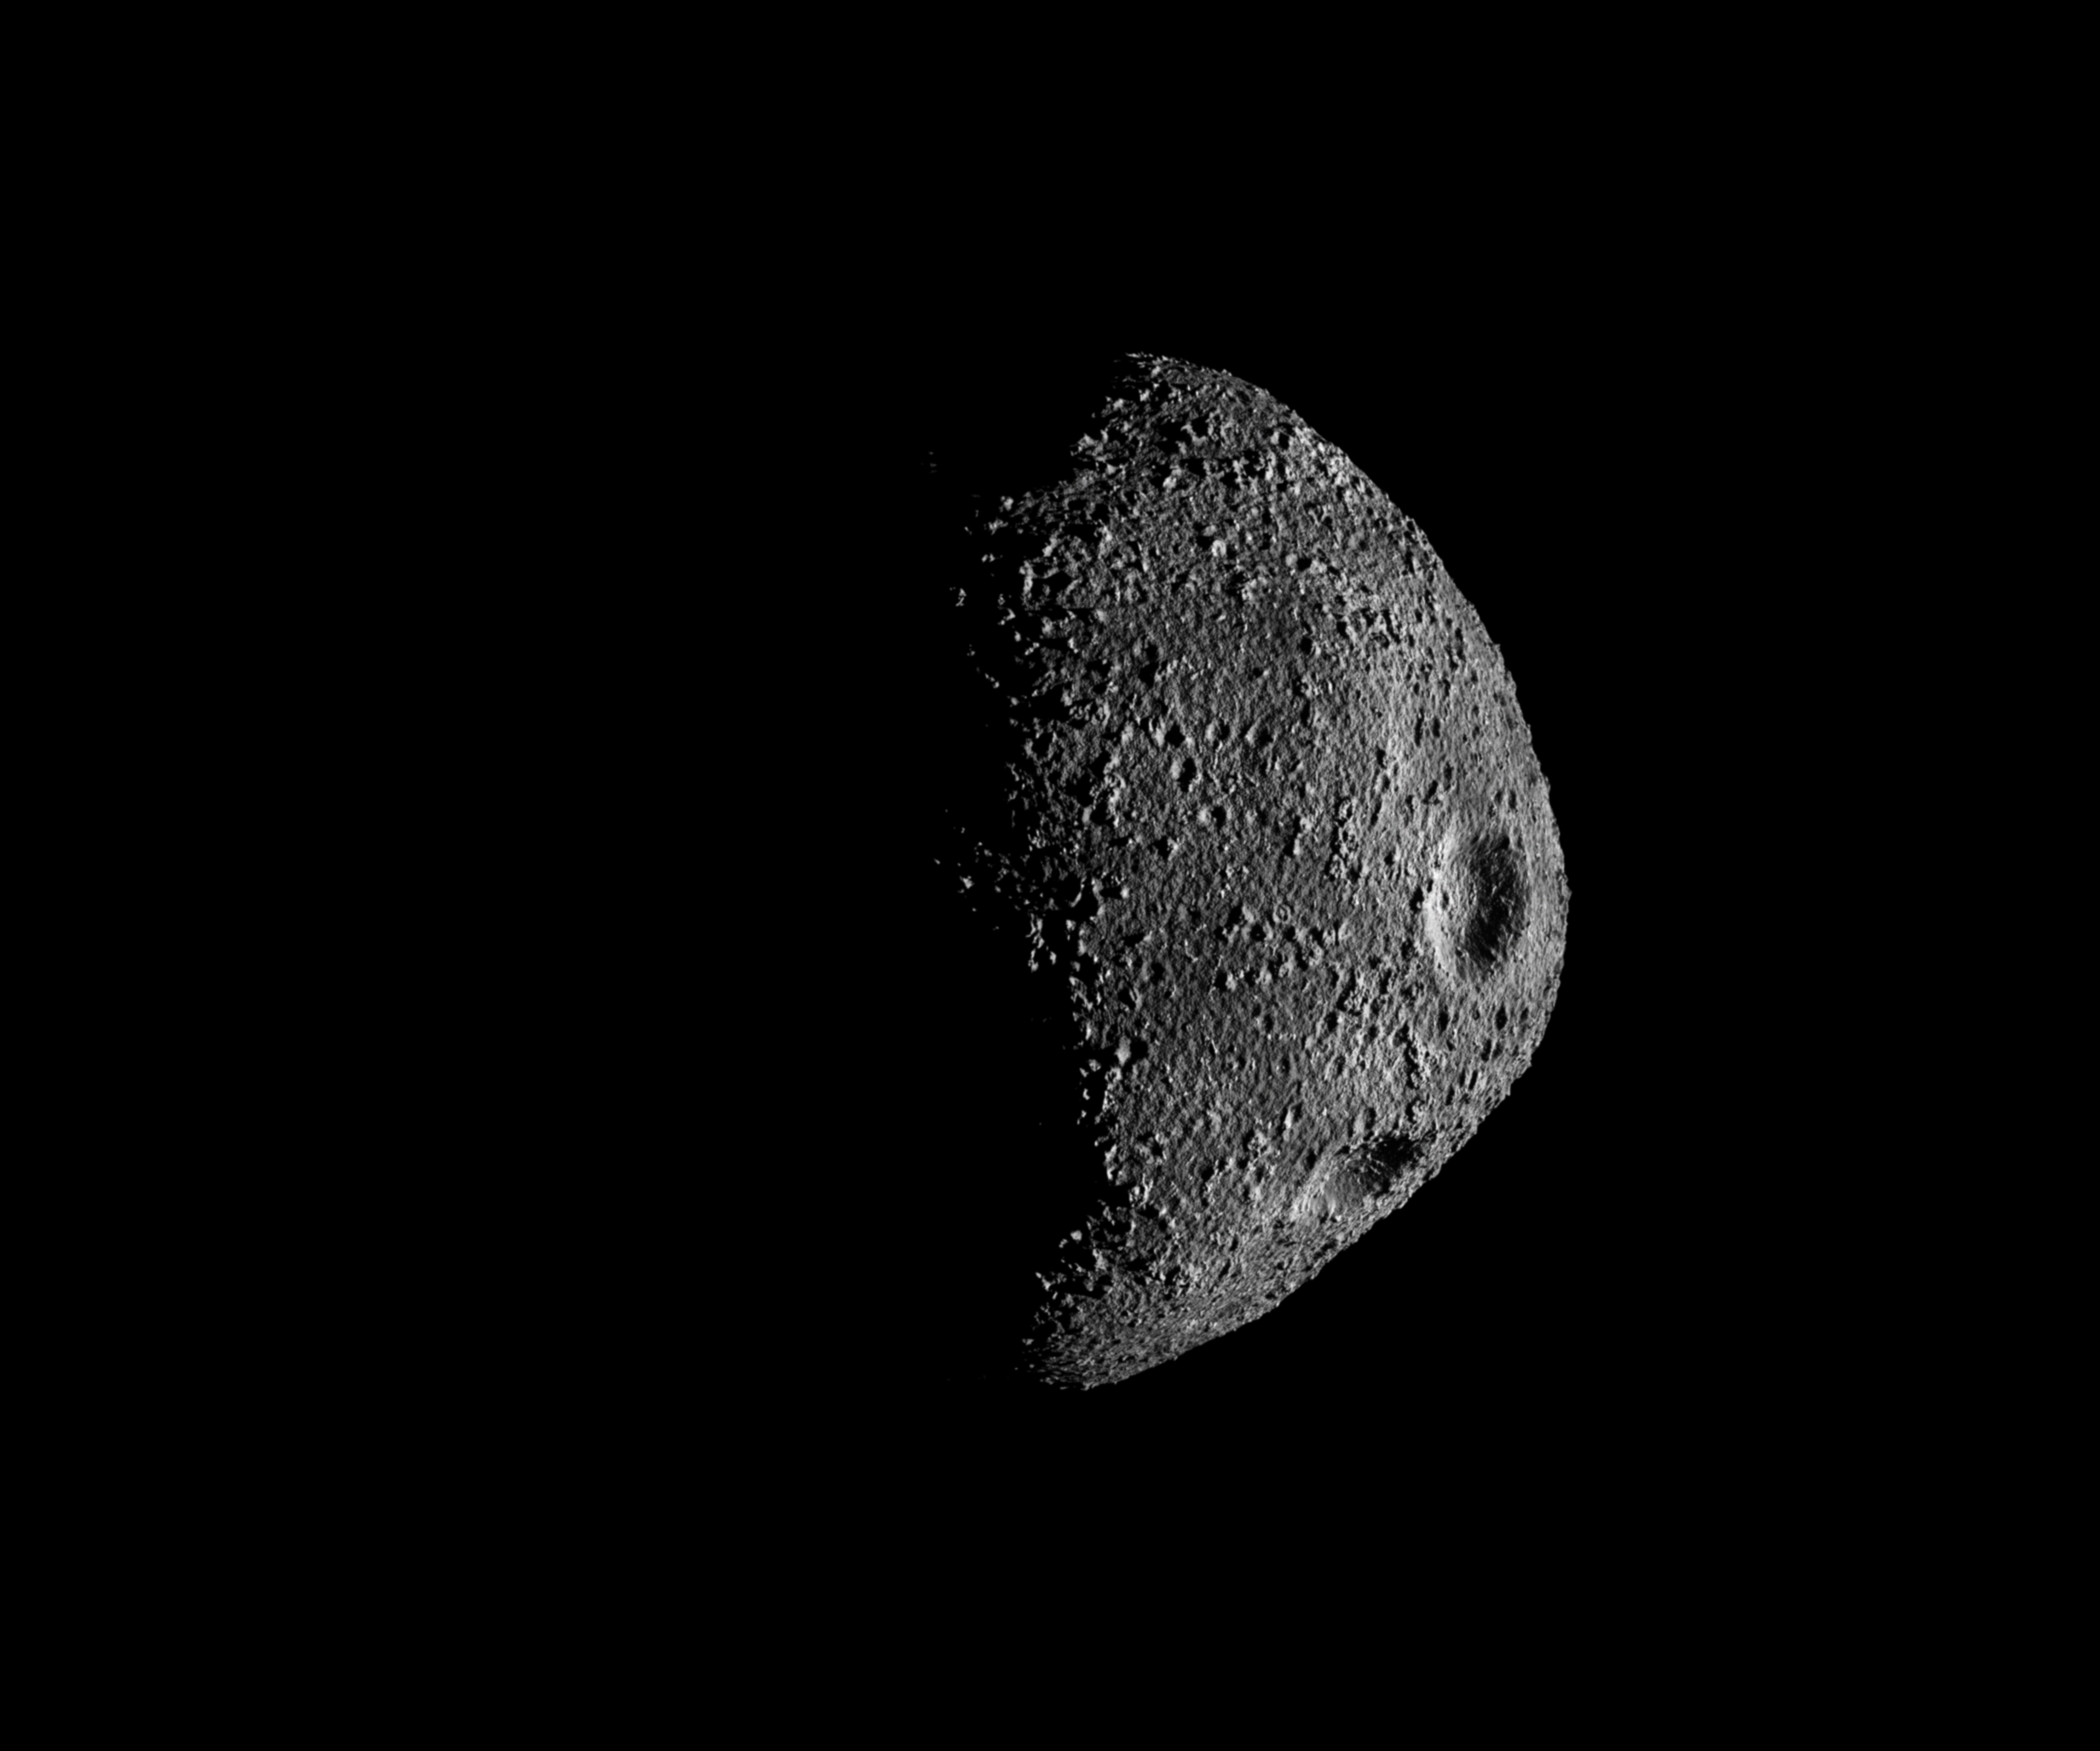
\includegraphics[width=\textwidth]{doc/thesis/0_figures/procedural_terrain/50_10_Inst_2017-08-15T115755-845000.png}
            \caption{\SI{400}{\kilo\meter}.}
            \label{fig:img_procedural_500}
        \end{subfigure}
        \\
        \begin{subfigure}[b]{0.75\textwidth}
            \centering
                \includegraphics[width=\textwidth]{doc/thesis/0_figures/procedural_terrain/50_10_Inst_2017-08-15T115855-260000.png}
            \caption{\SI{200}{\kilo\meter}.}
            \label{fig:img_procedural_100}
        \end{subfigure}
    \caption{Surface of a \SI{10}{\kilo\meter} \gls{sssb} for flybys with the given closest approach distance. Rendering artefacts, the ribbons, are clearly visible in both images.}
    \label{fig:img_procedural_10k}
\end{figure}

\subsection{Reconstruction}
\gls{sispo} is choosing which result of which reconstruction method to use based on the number of reconstructed points. Comparing the chosen algorithm with the input parameter reveals that the first incremental \gls{sfm} reconstruction performs better when the flyby distance is smaller while the second incremental \gls{sfm} algorithms performs better with farther flyby distances.

\begin{table}[htb]
    \centering
    \caption{Reconstruction Settings}
    \label{tab:comp_settings}
    \begin{tabular}{l|l}
        \textbf{Parameter Name} & \textbf{Value} \\ \hline
        export\_type       & obj   \\
        focal & 66667 \\
        cam\_model & \SI{1}{}     \\
        geo\_model & \SI{10}{\kilo\meter\per\second} \\
        num\_overlaps  & \SI{4}{} \\
        use\_prior & \SI{1}{} \\
        use\_upright & \SI{0}{} \\
        force\_compute & \SI{0}{} \\
        descriptor & SIFT \\
        d\_preset & ULTRA \\
        method & FASTCASCADEHASHINGL2 \\
        refine\_options & NONE \\
        reduce\_memory & 1
    \end{tabular}
\end{table}

\subsection{Performance}
\gls{sispo} was executed on a machine running Linux Ubuntu 18.04.03 LTS, \SI{16}{\giga\byte} of \gls{ram}, Intel\textsuperscript{\textregistered}~Core\texttrademark~i7-8700 processor with \SI{6}{} cores and an NVIDIA\textsuperscript{\textregistered}~GeForce GTX 1080 with \SI{8}{\giga\byte} memory. The performance assessment of a complete \gls{sispo} run shows that the most time consuming part is rendering. 
A test case with an encounter distance of \SI{50}{\kilo\meter}, a relative velocity of \SI{30}{\kilo\meter\per\second} and \SI{120}{} images is investigated. The complete statistics are presented in Appendix \ref{sec:app_performance}. The total execution time is \SI{41849.938}{\second}. The time spent rendering is \SI{40617.382}{\second}, approximately \SI{97}{\percent} of the overall total. The time spent reconstructing was \SI{785.949}{\second}, approximately \SI{2}{\percent} of the overall total. Hence, the Python code was not improved to reduce execution time since \SI{99}{\percent} of the execution time stem from time spent outside the Python code.